\begin{figure}[!h] 
\centering
\subfigure[With Mac FaceTime HD Camera]{
  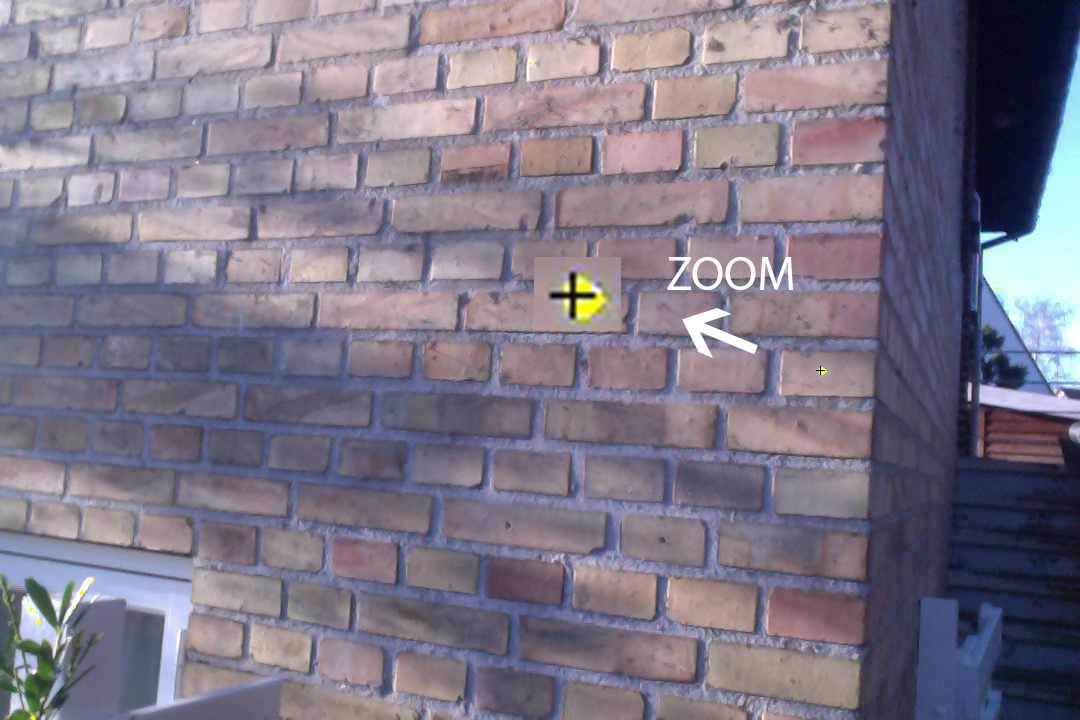
\includegraphics[scale=0.18]{fig/CentroidFrameOutdoor.png}
  \label{fig:outdoor}
}
\quad 
\quad 
\subfigure[With the Webcam Philips]{
  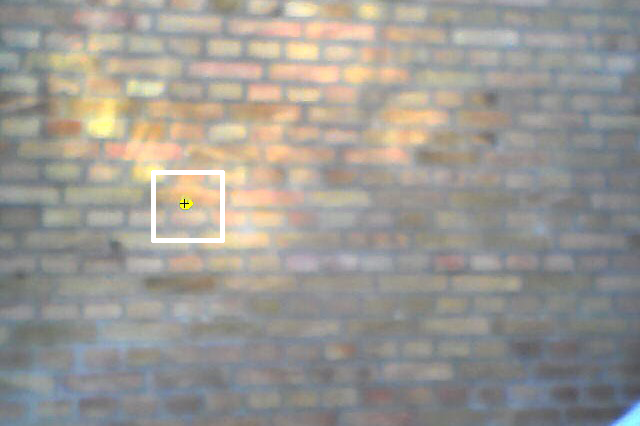
\includegraphics[scale=0.3]{fig/CentroidFrameOutdoorBlurred.png}
  \label{fig:outdoorBlurred}
}
\caption{Images Acquired by the Two Different Cameras Outdoor With Sunlight} 
\end{figure}

The two first experiments were carried out indoor. Thus, the sunlight was not taken into account, which is quite problematic since it could make impossible the color detection as the green beam will be as bright as the sun rays on the surface. In order to check if despite the sunlight, the color detection algorithm would be capable of detecting the laser or LED beam spot on Mars, it is experimented on Earth since the sun has similar features. As the webcam used during the experiment blurs the image, another picture is acquired to make sure that it works in the two cases. The images of the test, taken around 11 am during a sunny day, are shown on figures \ref{fig:outdoor} and \ref{fig:outdoorBlurred}.

The experiment is quite conclusive. The HSV parameters were tuned and it was difficult since the spots are small and could be mistaken as noise. However, it was feasible, as it can be noticed on the figures, where the centroid is displayed in black. It is on the point even if in the first image, it is not in the center of mass because the size of the point was reduced by decreasing the noise. Since the Signal Noise Ratio on Earth with the Sunlight as noise should be similar to the one on Mars, it can be deduced that the detection of the artificial light beam spots is achievable.